\qquad	 В методичці "Вивчення радіоелектронних схем методом комп'ютерного моделювання" можна знайти схему, що допомагає нам отримати значення сили струму на ділянці кола і напругу на діоді. Для складання цієї схеми нам необхідно використати наступні компоненти: \par
\indent \hspace{1em} резистор опором 10 Ом, \newline
\indent \hspace{1em} діоди BH01Pasd, \newline
\indent \hspace{1em} XSC1 - осцилогаф,\newline
\indent \hspace{1em} XFG1 - функціональний генератор,\newline
\indent \hspace{1em} ключі K1, K2, K3.\par
Переключаючи ключі, можемо отримати ВАХ для кожного з діодів а також їх комбінацій.
\begin{figure}[ht]

\centering

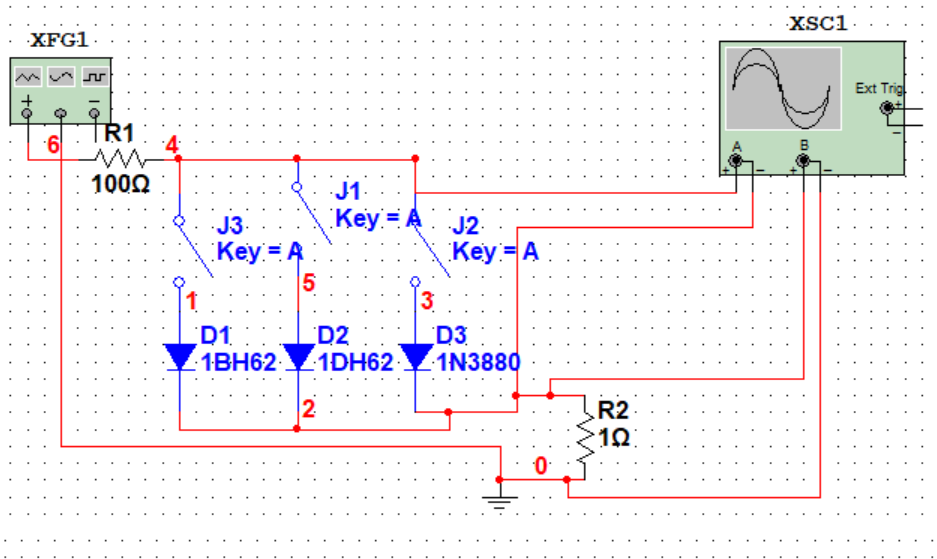
\includegraphics[width=0.8\linewidth]{Схема.png}

\caption{CСхема, що використовувалась у роботі}

\label{fig:mpr}

\end{figure}
